\documentclass[a4paper]{article}

%use the english line for english reports
%usepackage[english]{babel}
\usepackage[portuguese]{babel}
\usepackage[utf8]{inputenc}
\usepackage{indentfirst}
\usepackage{graphicx}
\usepackage{verbatim}
\usepackage{listings}
\usepackage{float}

\begin{document}

\setlength{\textwidth}{16cm}
\setlength{\textheight}{22cm}

\title{\Huge\textbf{Título do Trabalho}\linebreak\linebreak\linebreak
\Large\textbf{Relatório Intercalar}\linebreak\linebreak
\linebreak\linebreak

\includegraphics[scale=0.1]{feup-logo.png}\linebreak\linebreak
\linebreak\linebreak
\Large{Mestrado Integrado em Engenharia Informática e Computação} \linebreak\linebreak
\Large{Programação em Lógica}\linebreak
}

\author{\textbf{Grupo xx:}\\
José Pedro Borges - up201503603 \\
Miguel Mano Fernandes - up201503538 \\
\linebreak\linebreak \\
 \\ Faculdade de Engenharia da Universidade do Porto \\ Rua Roberto Frias, s\/n, 4200-465 Porto, Portugal \linebreak\linebreak\linebreak
\linebreak\linebreak\vspace{1cm}}

\maketitle
\thispagestyle{empty}

%************************************************************************************************
%************************************************************************************************

\newpage

%Todas as figuras devem ser referidas no texto. %\ref{fig:codigoFigura}
%
%%Exemplo de código para inserção de figuras
%%\begin{figure}[h!]
%%\begin{center}
%%escolher entre uma das seguintes três linhas:
%%\includegraphics[height=20cm,width=15cm]{path relativo da imagem}
%%\includegraphics[scale=0.5]{path relativo da imagem}
%%\includegraphics{path relativo da imagem}
%%\caption{legenda da figura}
%%\label{fig:codigoFigura}
%%\end{center}
%%\end{figure}
%
%
%\textit{Para escrever em itálico}
%\textbf{Para escrever em negrito}
%Para escrever em letra normal
%``Para escrever texto entre aspas''
%
%Para fazer parágrafo, deixar uma linha em branco.
%
%Como fazer bullet points:
%\begin{itemize}
	%\item Item1
	%\item Item2
%\end{itemize}
%
%Como enumerar itens:
%\begin{enumerate}
	%\item Item 1
	%\item Item 2
%\end{enumerate}
%
%\begin{quote}``Isto é uma citação''\end{quote}


%%%%%%%%%%%%%%%%%%%%%%%%%%
\section{O Jogo Oolong}

Oolong é um jogo de tabuleiro desenvolvido em 2015 pelo artista John Shulters e designer Sarah Graybill e publicado por Black Straw Games.
Trata-se de um jogo de estratégia para dois jogadores situado numa casa de chá japonesa. Cada jogador representa um fabricante de chá (preto e verde) tentando servir o máximo da sua marca. Quando um jogador servir 5 porções numa mesa, haverá atingido a maioria nessa mesa. Vencer o jogo envolve atingir a maioria em 5 mesas e, consequentemente, na casa.

São requeridos os seguintes componentes para iniciar um jogo:
\begin{itemize}
\item 80 peças - 40 pretas e 40 verdes
\item 8 marcadores especiais quadrados
\item 9 mesas redondas
\item 1 peão de empregado de mesa
\end{itemize}

A organização das 9 mesas deverá seguir a seguinte estrutura: \newline \newline
\begin{center}
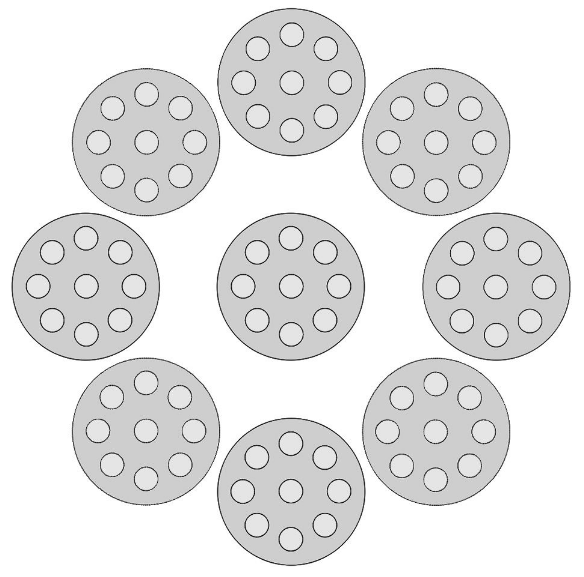
\includegraphics[scale=0.5]{board-setup.png}\linebreak\linebreak
\end{center}

Como cada uma das 9 mesas tem 9 posições para jogar será mais fácil imaginar uma bússola por cima do tabuleiro em que cada lugar na mesa e cada mesa representam uma direção (N, NE, E, SE, S, (...) e centro). 

\subsection{Regras do Jogo}
\subsubsection{Começar o jogo}
Quem começa o jogo é o jogador com o chá preto e tem de colocar uma das peç
as dele na mesa do centro, em qualquer posição. Se os jogadores estiverem envolvidos em múltiplos jogos, quem começa é quem perdeu o último. Cada jogada envolve colocar uma peça, mover o empregado e, possivelmente, ativar uma Ação Especial.

\subsubsection{Colocação de peças}
O lugar em que a peça é colocada indica a mesa em que se vai jogar a seguir. Por exemplo, se o jogador Verde jogar no lugar SE da mesa do centro, o jogador Preto tem de jogar na mesa SE do tabuleiro, na posição que quiser, desde que não esteja já ocupada. Se ele jogar na posição NE, o outro jogador tem de jogar na mesa NE e por aí adiante.

\subsubsection{Mover o empregado}
O empregado é utilizado para ajudar a saber onde vai ser colocada a próxima peça e onde estava anteriormente. As regras de utilização são as seguintes:
\begin{itemize}
\item Quando é jogada uma peça, o empregado é movido para a mesa onde vai ser feita a próxima jogada.
\item Ao colocar o empregado é preciso ter o cuidado de o pôr na peça que represente a mesa onde foi jogado o turno anterior.
\end{itemize}
Por exemplo, se o jogador Preto está na mesa do centro e joga na posição W, é preciso colocar o empregado na mesa W e na posição do centro desta.

\subsection{Marcadores especiais}
Existem 8 marcadores especiais que são designados aleatoriamente às mesas (Cada mesa só tem um no máximo). Cada marcador tem um efeito diferente e são ativados imediatamente mal o requisito que eles exigem seja feito. Após a ação ter sido feita não poderá voltar a ser usado até ao final do jogo. Se uma ação ativar outra ação noutra mesa, esta também será executada, ou seja, é permitido encadeamento de ações especiais.


\begin{minipage}[t]{0.1\textwidth}
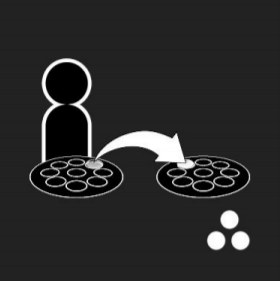
\includegraphics[scale=0.25]{black-move.png}
\end{minipage}
\begin{minipage}[t]{0.3\textwidth}
O jogador preto pode mover uma das suas peças de uma mesa não conquistada para uma outra mesa qualquer não conquistada. \textbf{Requisito:} 3 peças iguais.
\end{minipage}

\begin{minipage}[t]{0.1\textwidth}

\includegraphics[scale=0.25]{green-move.png}
\end{minipage}
\begin{minipage}[t]{0.3\textwidth}
O jogador verde pode mover uma das suas peças de uma mesa não conquistada para uma outra mesa qualquer não conquistada. \textbf{Requisito:} 3 peças iguais.
\end{minipage}

\begin{minipage}[t]{0.1\textwidth}
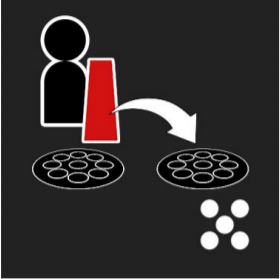
\includegraphics[scale=0.25]{black-waiter.png}
\end{minipage}
\begin{minipage}[t]{0.3\textwidth}
O jogador preto pode mover o Empregado do espaço onde está para o mesmo espaço numa mesa diferente. \textbf{Requisito:} 5 peças iguais.
\end{minipage}

\begin{minipage}[t]{0.1\textwidth}
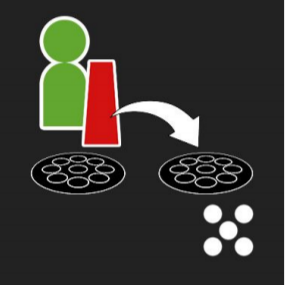
\includegraphics[scale=0.25]{green-waiter.png}
\end{minipage}
\begin{minipage}[t]{0.3\textwidth}
O jogador preto pode mover o Empregado do espaço onde está para o mesmo espaço numa mesa diferente. \textbf{Requisito:} 5 peças iguais.
\end{minipage}

\begin{minipage}[t]{0.1\textwidth}

\includegraphics[scale=0.25]{rotate.png}
\end{minipage}
\begin{minipage}[t]{0.3\textwidth}
(x2)O jogador que ativa a ação pode rodar a mesa para uma orientação qualquer (O Empregado também roda). \textbf{Requisito:} 4 peças iguais.
\end{minipage}

\begin{minipage}[t]{0.1\textwidth}
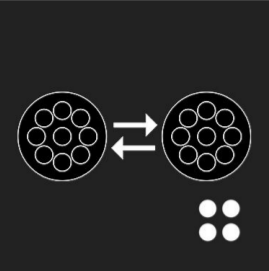
\includegraphics[scale=0.25]{swap-unclaimed.png}
\end{minipage}
\begin{minipage}[t]{0.3\textwidth}
O jogador que ativa a ação pode trocar a posição de duas mesas não conquistadas. O Empregado também é movido, se presente. \textbf{Requisito:} 4 peças iguais.
\end{minipage}

\begin{minipage}[t]{0.1\textwidth}
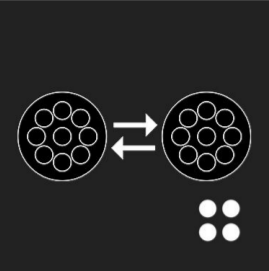
\includegraphics[scale=0.25]{swap-claimed.png}
\end{minipage}
\begin{minipage}[t]{0.3\textwidth}
O jogador que ativa a ação pode trocar a posição de duas mesas não conquistadas. O Empregado também é movido, se presente. \textbf{Requisito:} 5 peças iguais.
\end{minipage}


\subsection{Exemplo de uma sequência de jogadas}
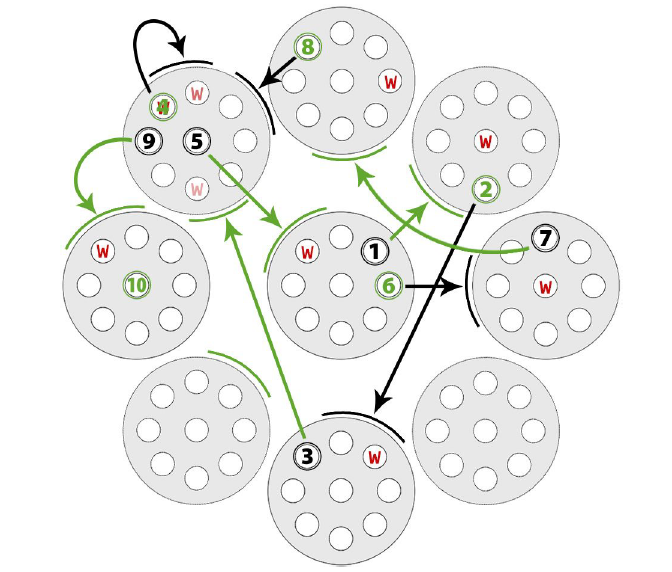
\includegraphics[scale=0.75]{board-jogadas.png}\linebreak\linebreak
\begin{enumerate}
\item Preto joga no espaço NE da mesa do centro e posiciona o Empregado(W) no centro da mesa NE.
\item Verde joga no espaço S da mesa NE e posiciona o Empregado no espaço NE da mesa S.
\item Preto joga no espaço NW da mesa S e posiciona o Empregado no espaço S da mesa NW.
\item Verde joga no espaço NW da mesa NW e posiciona o Empregado por cima da sua peça.
\item Preto joga no espaço do centro da mesa NW e posiciona o Empregado no espaço NW da mesa do centro.
\item Verde joga no espaço E da mesa do centro e posiciona o Empregado no espaço centro da mesa E.
\item Preto joga no espaço N da mesa E e posiciona o Empregado no espaço E da mesa N.
\item Verde joga no espaço NW da mesa N e posiciona o Empregado no espaço N da mesa NW.
\item Preto joga no espaço W da mesa NW e posiciona o Empregado no espaço NW da mesa W.
\item Verde joga no espaço centro da mesa W e irá posicionar o Empregado no espaço W da mesa do centro.
\end{enumerate}

\subsection{Conquistar uma mesa}
Quando um jogador tiver 5 peças da sua cor numa mesa, conquista essa mesa. A mesa pode continuar a ser utilizada nas jogadas, mas quando todos os espaços vazios forem preenchidos a mesa será considerada completa e qualquer jogada que levaria um jogador a ir para essa mesa será substituída, fazendo com que o jogador possa escolher um lugar qualquer vazio para colocar a sua peça.

\subsection{Fim do Jogo}
Quando um jogador conquista 5 das 9 mesas o jogo acaba imediatamente.

%%%%%%%%%%%%%%%%%%%%%%%%%%
\newpage
\section{Representação do Estado do Jogo}
A representação do estado do jogo não se poderá cingir apenas ao armazenamento do tabuleiro, dada a existência de elementos exteriores dinâmicos - as cartas especiais.

Para tal, considerou-se favorável a utilização de uma estrutura de dados adicional - uma lista que correlaciona os marcadores especiais e as mesas.

De facto, seria possível a reserva de um elemento extra na representação de cada mesa, mas por motivos de simplificação e facilidade de impressão do tabuleiro, dividiu-se em dois arrays distintos.

\subsection{Tabuleiro}
O tabuleiro é uma matriz multidimensional que preserva as 9 mesas redondas, mapeadas de forma similar ao teclado numérico de um telemóvel. Ilustrando,

\begin{itemize}
\itemsep0em
\item A \textbf{1ª posição} da matriz corresponde à mesa \textbf{Noroeste} (NW).
\item A \textbf{2ª posição} da matriz corresponde à mesa \textbf{Norte} (N).
\item A \textbf{3ª posição} da matriz corresponde à mesa \textbf{Nordeste} (NE).
\item A \textbf{4ª posição} da matriz corresponde à mesa \textbf{Oeste} (O).
\item A \textbf{5ª posição} da matriz corresponde à mesa \textbf{central}.
\item ...
\end{itemize}

A correspondência de cada posição da mesa a um ponto cardeal segue o mesmo padrão.

\subsubsection{Representação inicial do tabuleiro}
No estado inicial, todas as células estão vazias - representadas por \texttt{`x'}.
\begin{lstlisting}
  [[x, x, x, x, x, x, x, x, x],
   [x, x, x, x, x, x, x, x, x],
   [x, x, x, x, x, x, x, x, x],
   [x, x, x, x, x, x, x, x, x],
   [x, x, x, x, x, x, x, x, x],
   [x, x, x, x, x, x, x, x, x],
   [x, x, x, x, x, x, x, x, x],
   [x, x, x, x, x, x, x, x, x],
   [x, x, x, x, x, x, x, x, x]]
\end{lstlisting}

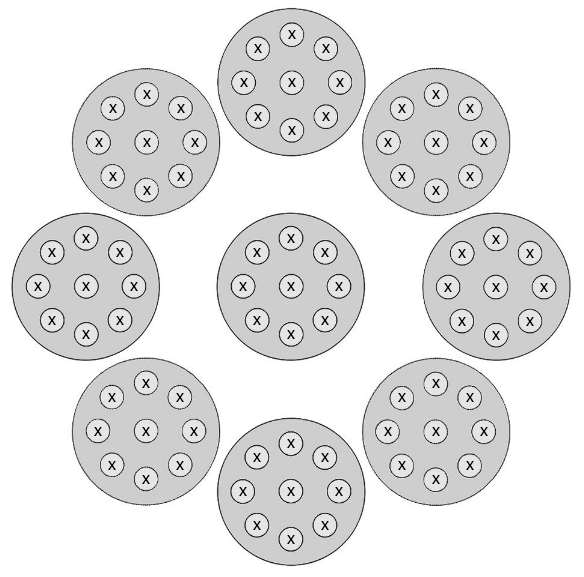
\includegraphics[scale=0.5]{board-setup-1.png}

\subsubsection{Representação intermédia do tabuleiro}
No estado intermédio, surge o aparecimento de peças pretas - representadas por \texttt{`b'} - e peças verdes - representadas por \texttt{`g'}.
\begin{lstlisting}
  [[x, g, x, x, x, b, x, x, x],
   [b, x, x, b, x, x, g, x, x],
   [x, b, x, x, b, x, x, g, x],
   [b, x, g, x, x, x, x, x, x],
   [x, x, b, x, x, b, x, x, g],
   [g, g, x, g, g, x, x, x, g],
   [x, x, x, x, x, b, x, x, x],
   [x, x, g, x, x, b, x, x, x],
   [x, x, x, x, x, b, x, b, x]]
\end{lstlisting}

Neste estado em específico ilustrou-se uma situação de vitória de mesa por parte do jogador verde. Note-se que a mesa Este - posição nº6 da matriz - acumula um total de 5 peças verdes, pelo que a maioria nesse ponto está estabelecida.

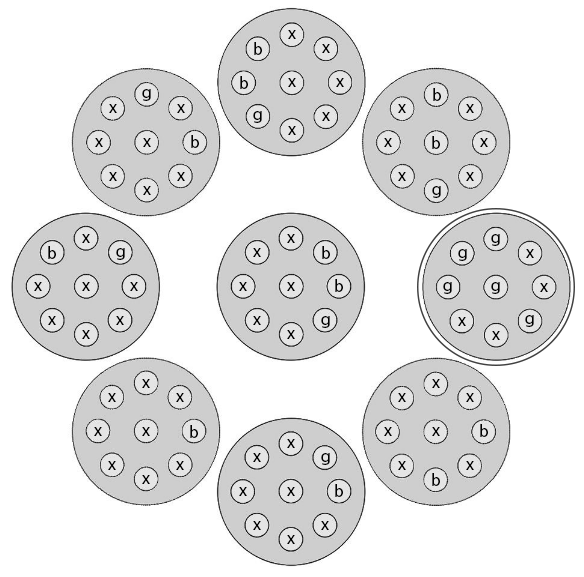
\includegraphics[scale=0.5]{board-setup-2.png}

\subsubsection{Representação final do tabuleiro}

\begin{lstlisting}
  [[g, g, b, b, b, b, g, g, x],
   [b, b, b, b, g, x, g, g, b],
   [g, b, x, g, b, x, g, g, g],
   [b, g, g, x, b, b, b, b, g],
   [b, g, b, g, x, b, b, b, g],
   [g, g, b, g, g, g, g, x, g],
   [b, x, b, b, g, b, x, b, g],
   [b, g, g, b, x, b, g, g, b],
   [g, b, x, g, g, b, b, b, b]]
\end{lstlisting}

Nesta situação final, o jogador preto emerge vitorioso, tendo conquistado maioria nas cinco mesas Norte, Oeste, central, Sudoeste e Sudeste. \newline

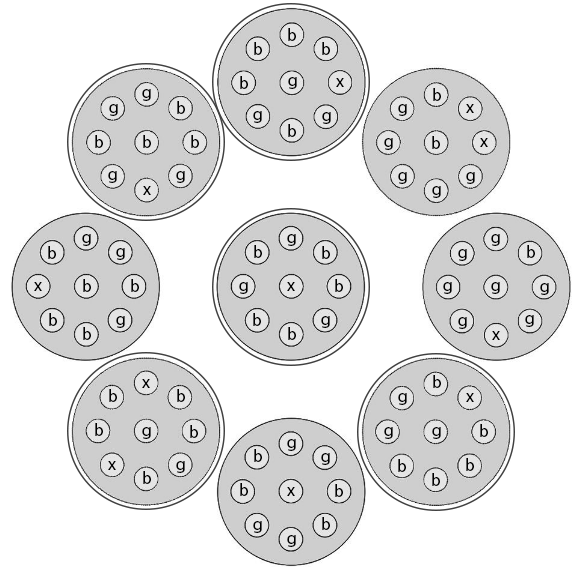
\includegraphics[scale=0.5]{board-setup-3.png}

\subsection{Marcadores especiais}
Dada a atribuição aleatória dos marcadores especiais - 8 na periferia, máximo de um por mesa - no início do jogo e a possibilidade do jogo terminar sem todos (ou até algum!) marcador ser consumido, apresentar-se-á apenas uma possível disposição inicial e intermédia/final.

O mapeamento continua a executar-se do mesmo método descrito anteriormente.

\subsubsection{Representação inicial dos marcadores}
\begin{lstlisting}
  [black_move, green_move, black_waiter, green_waiter, 
   empty, rotate, rotate, swap_unclaimed, swap_claimed]
\end{lstlisting}

Neste exemplo, o marcador \textbf{black\_move} está associado à mesa Noroeste.

Note-se a repetição da carta especial \textbf{rotate}, que efetivamente possui dois exemplares, e também a utilização da etiqueta \textbf{empty} para identificar mesas sem marcadores - ora consumidos, ora não atribuídos, como no caso da mesa central. \newline

\subsubsection{Representação intermédia/final dos marcadores}
\begin{lstlisting}
  [black_move, empty, black_waiter, green_waiter, 
   empty, rotate, rotate, empty, swap_claimed]
\end{lstlisting}

Nesta etapa do jogo, os marcadores \textbf{green\_move} e \textbf{swap\_unclaimed} haverão sido consumidos, daí a sua substituição por \textbf{empty}. \newline


%%%%%%%%%%%%%%%%%%%%%%%%%%
\section{Visualização do Tabuleiro}

A representação do tabuleiro em modo de texto não é feita com a disposição original do jogo para efeitos de simplificação. Em vez disso, é usada uma matriz de 3x3 mesas com 3x3 posições cada uma. As posições representam na mesma os pontos cardeais, para facilitar o jogo.

\begin{center}
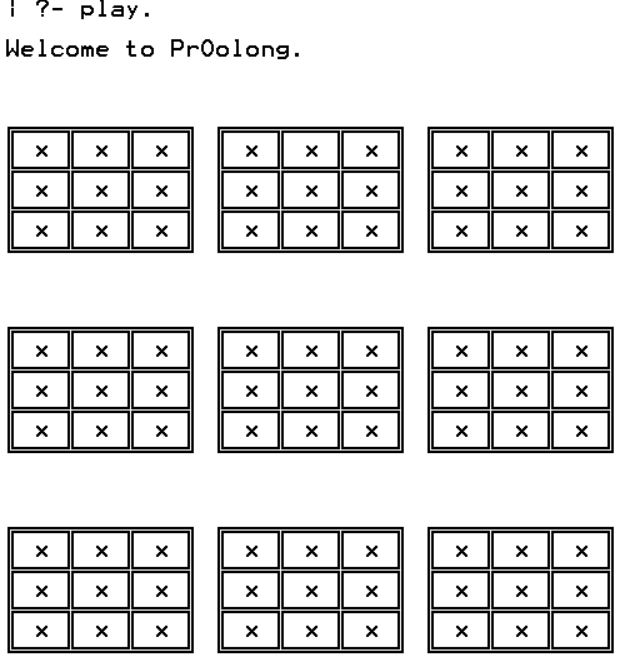
\includegraphics[scale=0.33]{tabuleiro.png}
\end{center}

Para produzir este efeito é usada o predicado \texttt{print\_formatted\_line(X)} para desenhar as linhas horizontais em cada matriz, que separam as posições. É usada várias vezes o predicado put\_code com os códigos ASCII 185, 187, 188, 201, 204, 205 e 206. X pode levar os argumentos 0, 1,2 ou 3 dependendo da linha a imprimir. Um dos usos do predicado é o seguinte:

\begin{lstlisting}
print_formatted_line(X) :- X = 1, 
  nl, put_code(204), put_code(205), put_code(205), put_code(205), 
  put_code(206), put_code(205), put_code(205), 
  put_code(205), put_code(206), put_code(205), put_code(205), 
  put_code(205), put_code(185), nl.
\end{lstlisting}

O predicado \texttt{print\_block([H|T])} junta o predicado acima com a impressão do array previamente definido. São usadas os predicados nh0, write, put\_code e print\_formatted\_line várias vezes para cada matriz permitindo desenhar o tabuleiro da forma que queremos.

\begin {lstlisting}
print_block([H|T]) :- nl, print_formatted_line(0), write(' '), 
  print_formatted_line(0),  write(' '), print_formatted_line(0), nl, 
  put_code(186), write(' '), nth0(0, H, E1), write(E1), write(' '), 
  put_code(186), (.....).
\end{lstlisting}

O predicado \texttt{print\_board([H|T])} é o chamado para imprimir tudo feito pelos predicados mencionados anteriormente.

\begin{lstlisting}
print_board([H|T]) :- length([H|T], Matrix_Size),
  Trim_Size is Matrix_Size - 3,
  trim_tail([H|T], Trim_Size, Block),
  print_block(Block),
  trim_head(T, 2, Remain),
  print_board(Remain).
\end{lstlisting}

\texttt{trim\_head(L,N,S)} remove N elementos da lista L e guarda o resultado em S. \texttt{trim\_tail(L,N,S)} faz o mesmo, só que em vez de cortar N elementos do principio, corta do fim


%%%%%%%%%%%%%%%%%%%%%%%%%%
\newpage
\section{Movimentos}

Cada turno, o jogador tem acesso a dois tipos de jogadas distintos:

\begin{itemize}
\item Colocação de uma peça em Board, enviando a posição de eleição numa lista cuja cabeça \textbf{H} corresponde à mesa e a cauda \textbf{T} à cadeira.

\texttt{place\_token([H|T], Board)}

\item Caso os requerimentos para a ativação de um marcador especial se cumpram, seleção de uma mesa \textbf{Table} do \textbf{Board} e ativação a sua habilidade.

\texttt{activate\_special(Table, Board)}
\end{itemize}

Note-se que o input adicional exigido ao jogador varia consoante o marcador selecionado. \newline

Por exemplo, o marcador \textbf{rotate} permite a rotação da mesa numa direção no sentido dos ponteiros do relógio ou inverso. Para tal, um possível predicado seria \texttt{rotate\_table(Direction, Table, Board)}. 	\newline

Traduzindo, a direção \textbf{Direction} - introduzida pelo jogador - da rotação da mesa \textbf{Table}, adquirida através do predicado \textbf{activate\_special}. Estas alterações manifestam-se em \textbf{Board}. \newline

Com o desenvolvimento do projeto e avanço da lógica de jogo, mais predicados deste género serão desenvolvidos.






\end{document}
